\chapter{Concept 2: State Machine Implementation}
\lhead{\thechapter \space Concept 2: State Machine Implementation}
\label{ch:concept_two}
Based on feedback received during the midterm presentation, it became clear that drastic changes needed to happen, mainly due to an improper requirements analysis. Since the concept described in chapter \ref{ch:concept_one} did not show promising results, it was decided to switch to a new concept in order to reduce the risk of not having a (partially) working product at the end. Through a brainstorm session with the company a new concept was developed. In order to combat time constraints, it was decided to limit the scope to just one side of a rack, instead of covering the whole warehouse. Further details regarding this concept are explained in the remainder of this chapter. Installation instructions and a guide for running the project can be found in appendix \ref{app:setup}.

\section{Product Functions}
\label{sec:product_description}
The goal of this project is mainly focused on developing a solution for providing a drone with collision avoidance. However, along the course of the project it became evidently clear that a indoor self-flying (figure \ref{fig:roadmap}) component was also necessary. From here on out, the functions could be divided among the 3 dimensions the drone has to interact with as follows:
\begin{figure}[h]
	\centering
	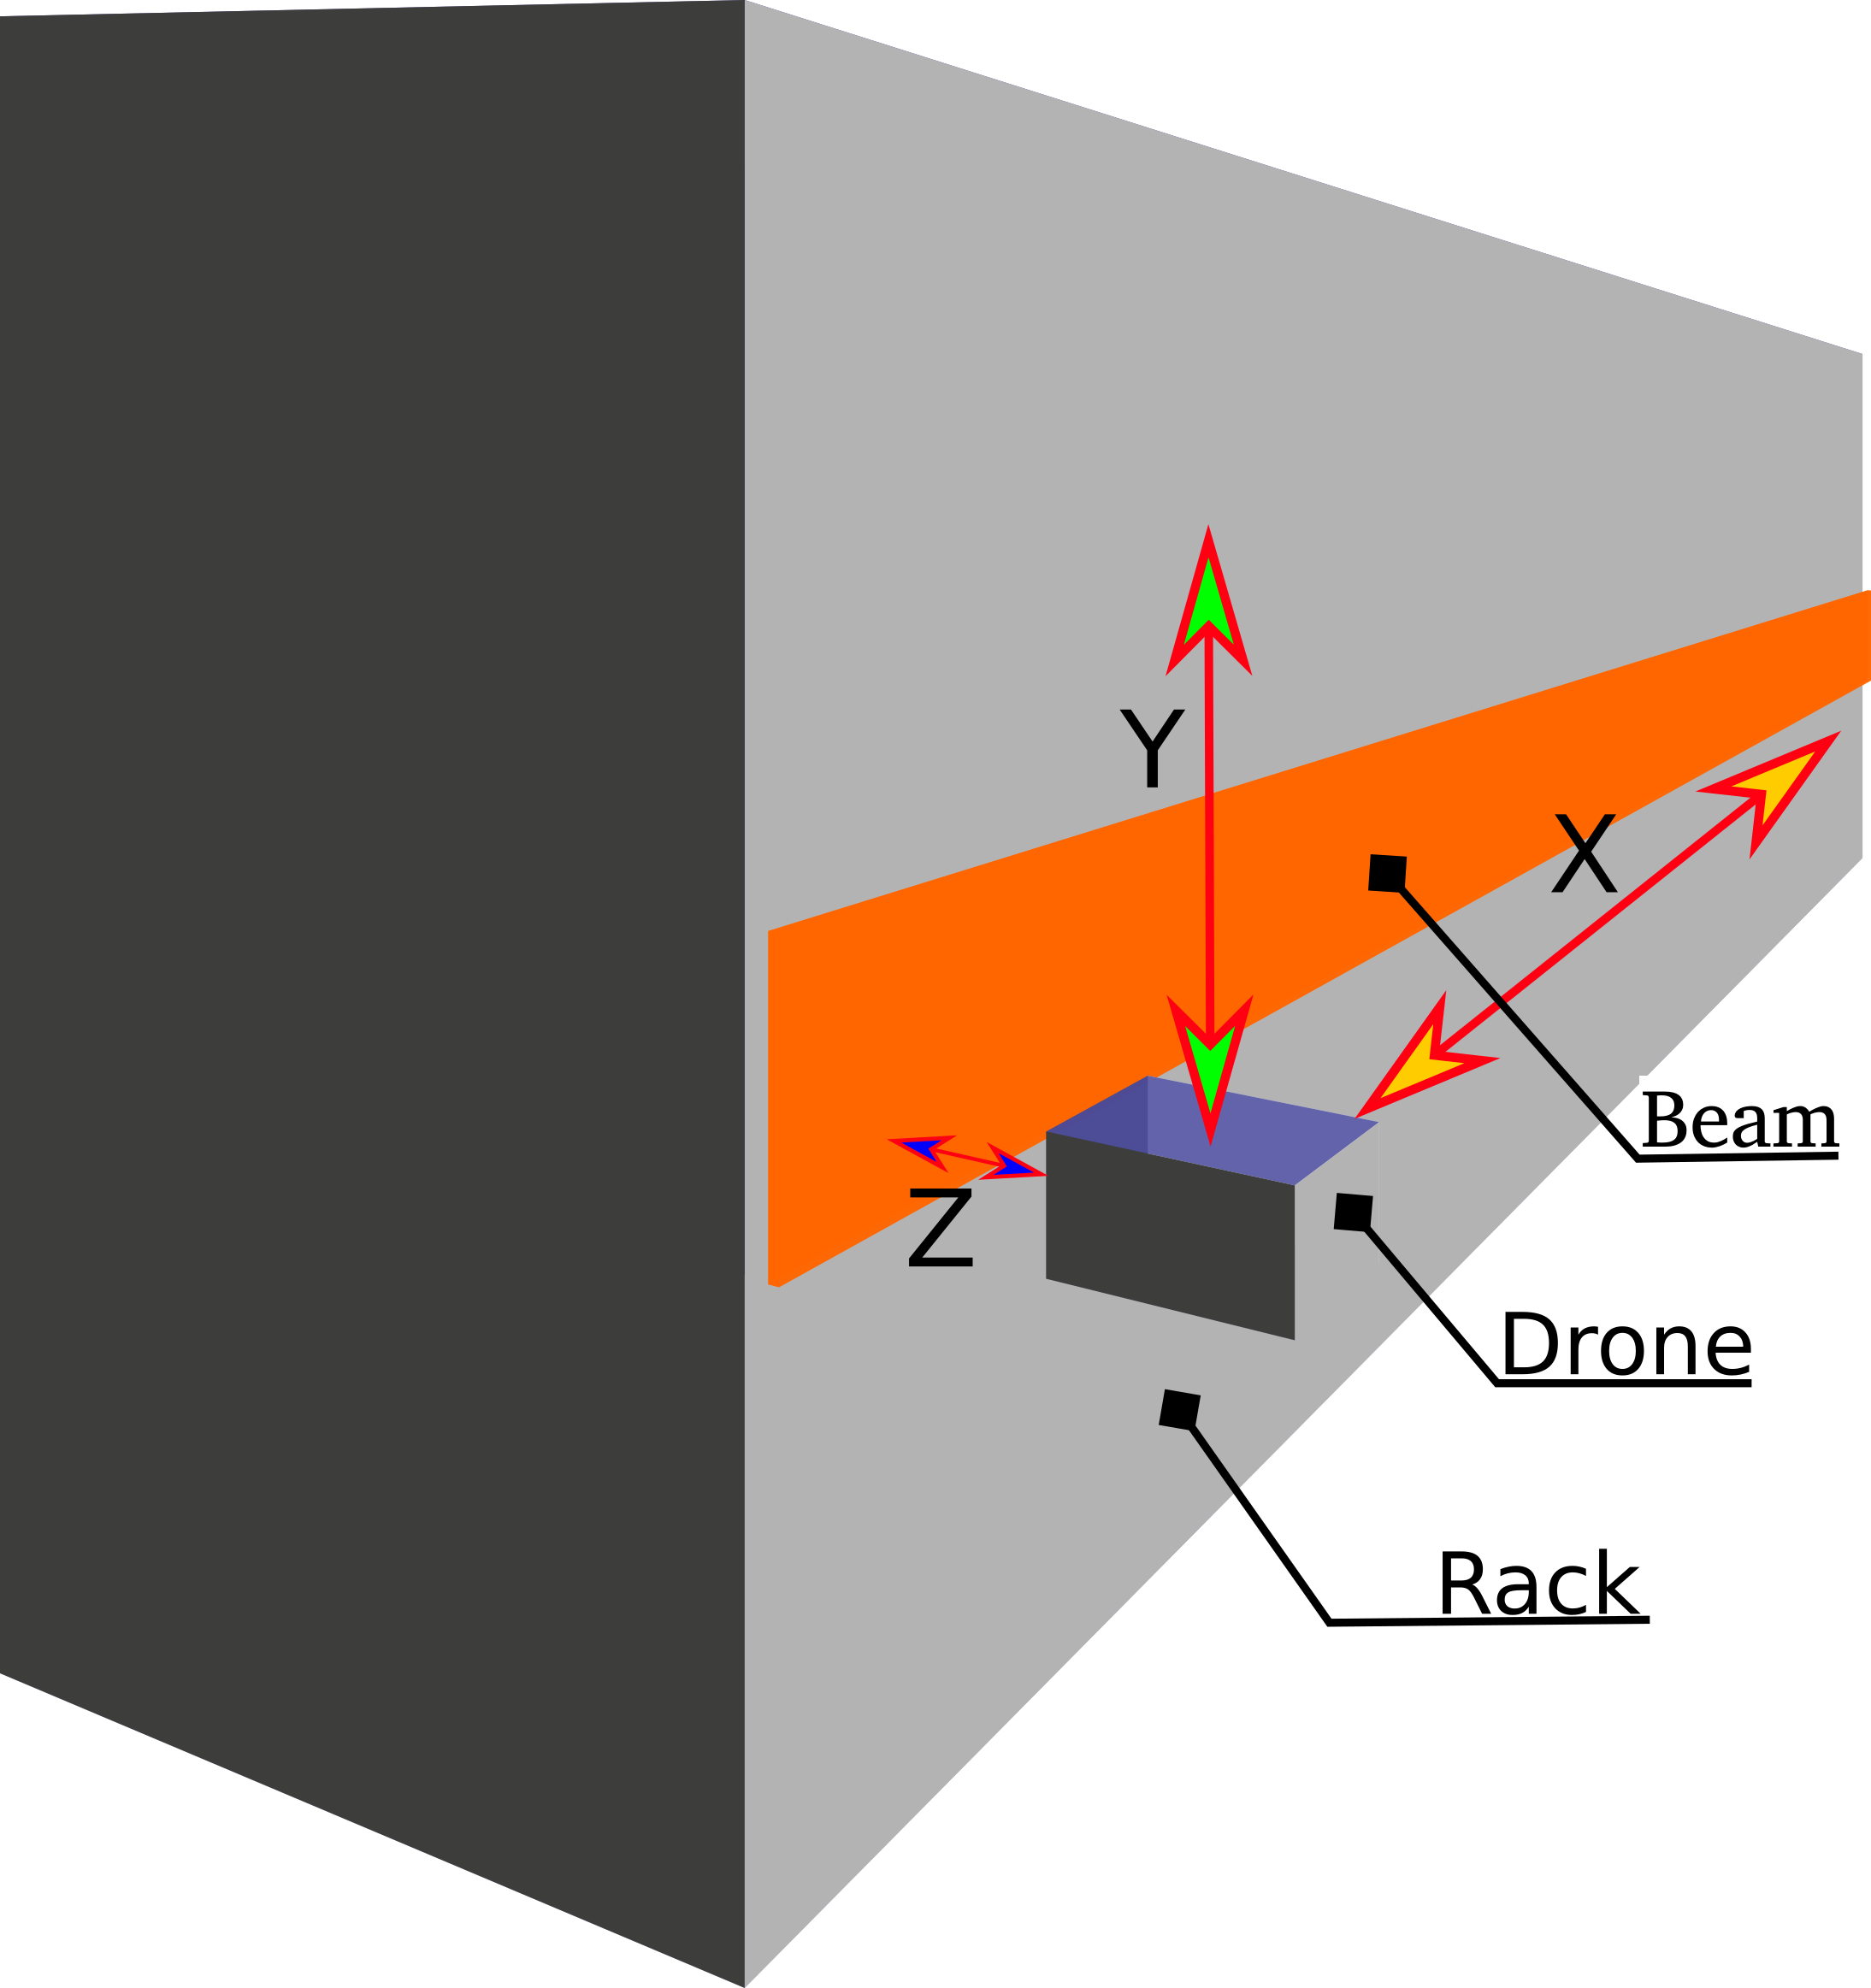
\includegraphics[width=\linewidth/2]{img/drone_concept_diagram}
	\label{fig:drone_concept}
	\caption{Visual representation of the single rack concept.}
\end{figure}

\begin{itemize}
	\item X-axis:
	\begin{itemize}
		\itemsep0em
		\item Move the drone sideways
		\item Stop the drone at the end of a bar
		\item Detect objects in the drone's trajectory
		\item Avoid collisions with objects in the drone's trajectory
	\end{itemize}
	\item Y-axis:
	\begin{itemize}
		\itemsep0em
		\item Keep the bar in the center of the drone's camera
		\item Change the drone's altitude to switch layers
		\item Keep track of the current layer and the highest layer
	\end{itemize}
	\item Z-axis:
	\begin{itemize}
		\itemsep0em
		\item Estimate the pixel size of the bar
		\item Keep the drone to maintain distance from the bar
	\end{itemize}
\end{itemize}
This list is originally taken from the \gls{SRS} in appendix \ref{app:srs}. Figure \ref{fig:drone_concept} contains a visual representation of the concept with its functions.

\section{State Machine}
The initial state design featured a concept where the drone correct its positions for safety, move sideways viewing the beam at set intervals and then do a check for objects in its trajectory. This design is displayed in appendix \ref{app:bar_states_simple}. However, it was decided to shift to a design that selects a state based on a set of criteria (see table \ref{tab:criteria}) so that states such as checking for collision or locking-on can happen more frequently. For the second state machine design, please refer to appendix \ref{app:bar_states_two}. It is important to note that as of writing this document, the states "moving layer" and "returning home" have not been implemented yet due to time constraints. The state "avoiding collision" has only been partially implemented, where it only determines if an object is too close and then proceeds to land accordingly. Descriptions of all implemented states can be found in table \ref{tab:state_desc}.
\begin{table}[h]
	\centering
	\resizebox{\textwidth}{!}{%
		\begin{tabular}{lll|l}
			\textbf{} &  &  & \textbf{Transition to state:} \\
			\textbf{Criteria:} & Locked on? & Distance interval reached? & \cellcolor[HTML]{9B9B9B}{\color[HTML]{333333} } \\ \hline
			& False & False & Locking on \\
			& False & True & Locking on \\
			& True & False & Advancing \\
			& True & True & {\color[HTML]{333333} Rotating to hall}
		\end{tabular}%
	}
	\caption{Table displaying state transitions from the facing bar state, based on 2 criteria.}
	\label{tab:criteria}
\end{table}

For simplification, the currently implemented state machine can be grouped into 3 group states: locking on, checking for collision, and advancing. Here, locking on refers to centering the beam in its view and maintaining an appropriate distance, checking for collision refers to rotating the drone to check the hallway for objects in its trajectory, and advancing refers to moving the drone sideways along the beam. The criteria "Locked on?" is currently set to false after having completed any of the aforementioned group states (aside from "locking on", which sets it to true again). "Distance interval reached?" is set to true after exiting the advancing group state, and back to false after exiting "checking for collision".

\begin{table}[h]
	\centering
	\resizebox{\textwidth}{!}{%
		\begin{tabular}{l|l}
			\textbf{State} & \textbf{Description} \\ \hline
			Facing beam & The drone is hovering in front of the beam while facing it. Also acts as a central state. \\
			Locking on & The drone is positioning itself to center the beam and maintain its distance from it. \\
			Advancing & The drone is moving sideways along the beam. \\
			Rotating hall & The drone is rotating towards to hall to prepare to check for collisions. \\
			Detecting collision & The drone is using background subtraction to check for objects in its near trajectory. \\
			Avoiding collision & The drone determines if an object is too close and lands to avoid collision if necessary. \\
			Rotating beam & The drone rotates back so it is once again facing the beam.
		\end{tabular}%
	}
	\caption{Implemented states with descriptions of what happens during their executions.}
	\label{tab:state_desc}
\end{table}

\section{Implementation}
\label{sec:implementation_two}
The implementation is written in Python and makes use of 3 main components: OpenCV, transitions, and the Tello-openpose project. OpenCV is a computer vision library \citep{opencv}, transitions is a Python package that provides state machine implementation functionality \citep{transitions}, and Tello-openpose is a project by Github user Geaxgx that enables a Tello drone to track a human and follow commands via gestures \citep{tello_openpose}. The last component mentioned was used as the basis for this project, but has since been modified significantly.
\\\\
The product contains the following scripts with the following responsibilities:

\paragraph{Main.py:} Used to run the product, primarily responsible for invoking the other scripts, connecting to the drone, and running a loop to obtain the frames.

\paragraph{DroneController.py:} Communication script between the other scripts and the drone. It stores information about the drone, handles the logs, and provides functionality for controlling the drone either through functions or by keyboard. This script was based on the Tello-openpose project, and makes use of a Python package called Tellopy that provides a set of functions for the scripted controlling of a Tello drone \citep{tellopy}.

\paragraph{BeamDetector.py:} Provides functions that get an estimate of the edges of a beam. This happens by using OpenCV to get a binary (either black or white pixels) image, get the contours, and then obtain all straight lines from the contours using a function called \gls{houghLinesP}. To filter out noise, the script also gets the average Y-coordinate of all lines to create a pivot, and then groups them together into a lower-half and upper-half group. The respective averages of those 2 groups then form the upper-edge and lower-edge of the beam.

\paragraph{DistanceEstimator.py:} Provides functions for getting the distance between the center of the beam and the camera center, as well as a function for estimating the distance based on the size of the beam in pixels. The former is done by providing the frame width, frame height, and the minimal and maximal Y-coordinate found using the functions of BeamDetector.py.

\paragraph{CollisionDetector.py:} Provides functions that can distinguish foreground objects from background objects, get the contour size from the foreground objects and use that to very roughly estimate the proximity based on the amount of space the contour takes up in the frame. For reference, please look at figure \ref{fig:collision_detection}. The top two images are frames directly from the drone camera, and the bottom two are the same frames where background subtraction has been applied. In the images of the left column the drone is at a safe distance, while in the right column it is too close, hence why the bottom right image has a "Danger" tag in it.

\paragraph{StateMachine.py:} Makes use of the transitions Python package to define the states, the possible state transitions, and the conditions for transitioning. Also stores a time stamp of the time when the most recent state enter has occurred.
\begin{figure}[h]
	\centering
	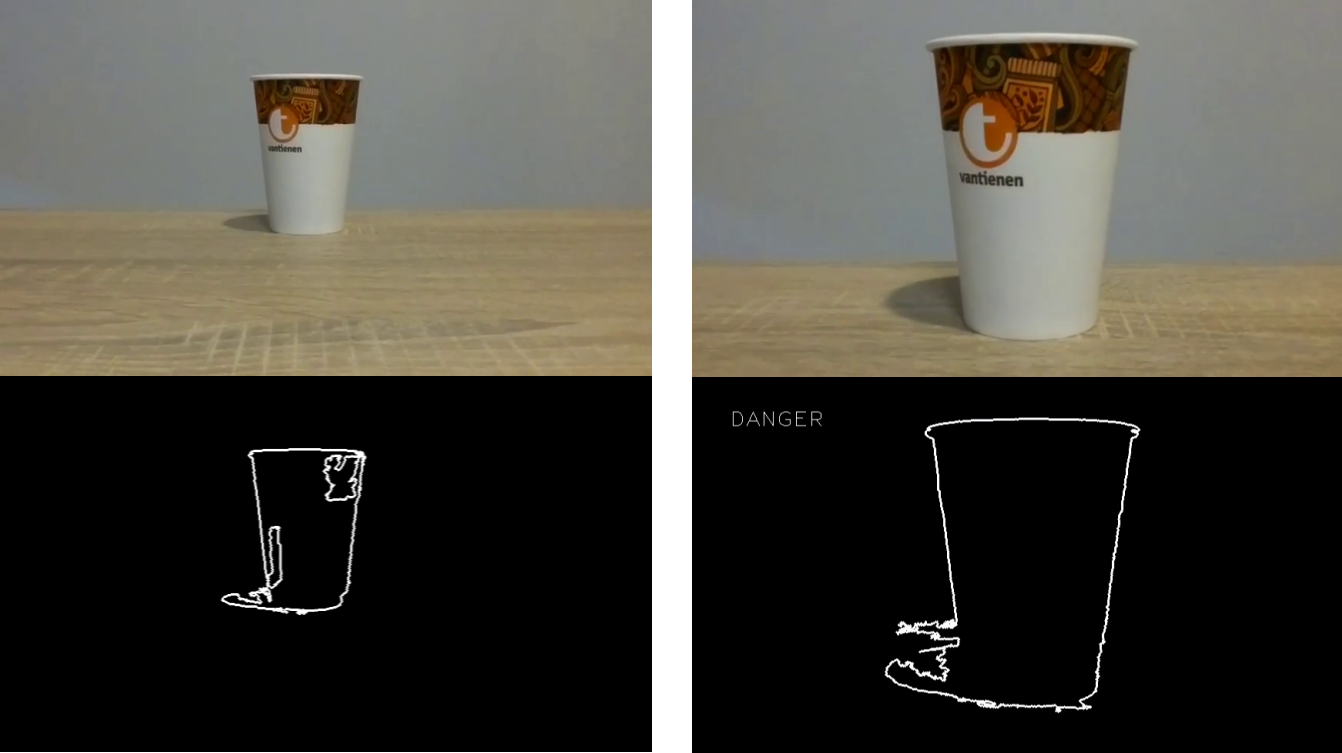
\includegraphics[width=\linewidth]{img/collision_detection_sample}
	\label{fig:collision_detection}
	\caption{Set of images demonstrating collision detection.}
\end{figure}

\paragraph{StateMachineActions.py:} Acts as a bridge between StateMachine.py and DroneController.py. It has an execute function that checks the state of the StateMachine instance and invokes a function accordingly. It also checks when a state can be exited, and updates the criteria seen in table \ref{tab:criteria}. For example, when the StateMachine instance has entered the "advancing" state, StateMachineActions will invoke the function in DroneController that will make the drone move sideways until the interval is reached. Then it will update the criteria and use the transition to go back to the "facing bar" state.

\paragraph{FPS.py \& HUD.py:} As Main.py displays the camera frames in a window, HUD.py adds and updates textual information to each frame. FPS.py calculates the frames per second, which is in turn used by HUD.py. The code of both these scripts originated from the Tello-openpose project.
\pagebreak
\section{Limitations \& Problems}
\label{sec:state_machine_limits}
The current product faces 2 major issues. The biggest issue is the limitations of classical computer vision algorithms, on which the product is highly dependent on. A lot of averaging has been done in an attempt to minimize noise, however it seems that the distance and lighting range in which the product operates normally is still rather small. Another major issue is the communication with the current drone. It only accepts one command at a time sent by an UDP-protocol ("single shot" message-oriented communication protocol), which might cause the software and the drone to desynchronize. To clarify, listing \ref{lst:error_log} displays the debug log while running the Main.py script. Each 0.2 seconds the current state is printed. However, while in line 2 and 3 it shows the command is received by the drone fairly quickly after switching states (at least within 0.2 seconds), it does not to seem to be the case when rotating back at lines 6-8. This causes the drone to not rotate back all the way (due to the duration of the rotation being an estimate based on speed and distance) and ultimately causes it to stop functioning properly.
\begin{lstlisting}[caption={Fragment excerpted from the debug log of the product.},captionpos=b,label={lst:error_log}]
facing bar
Rotating to hall
Tello: 14:44:45.588:  Info: clockwise(val=100)
...
Avoiding collision
Rotating to bar
Rotating to bar
Tello: 14:44:48.224:  Info: clockwise(val=-100)
Rotating to bar
Stopping rotation
Tello: 14:44:48.494:  Info: clockwise(val=0)
facing bar
\end{lstlisting}

One minor improvement point is that the distance between the camera center and the center of the beam is still measured in pixels, while the distance between the drone and the beam is in metric units. For consistency purposes, this should be changed to the same format.
\\\\
There are also a couple of limitations caused by the Tello drone. To be able to stabilize itself, it makes use of an infrared camera that points to the surface it is hovering over. However, the requirements for this to work are rather strict. It seems to respond badly to uneven surfaces (think of flying over small objects such as doorsteps), reflective surfaces, and dark or monochrome surfaces. The issue with this is that, especially in the case of uneven surfaces, the drone will force itself to correct its position, and thus overrule any other input. This might cause issues when a drone were to fly over a box on the ground at a low altitude as the script receives very little information about the drone's status, causing it to ultimately desynchronize. Another limitation is its battery life, which, after testing, spans roughly 10 minutes.

%TODO:add class diagram?
%TODO: Elaborate on computer vision pipeline